\section{Project description}
\label{chapter1}

\subsection{Problem desription}

When the CO2 level in a room reaches a certain level, a window should automatically open and a fresh air fan should switch on.
After a certain lower CO2 level is reached and a certain run-on time has elapsed, the window is closed again and the fan is switched off again.

\subsection{Hardware}

\begin{enumerate}[label*=\arabic*.]
    \item \label{hw.1} MH-Z19 CO2 Sensor 
    \item \label{hw.2} Arduino with bluetooth module 
    \item \label{hw.3} Raspberry 
    \item \label{hw.4} Electric motor
\end{enumerate}

\subsection{Hardware}

\begin{enumerate}[label*=\arabic*.]
    \item \label{io.1} Analog input for measuring the CO2 contentr 
    \item \label{io.2} Digital output for controlling a window opener 
    \item \label{io.3} Digital output to control a fan 
\end{enumerate}

\subsection{Schema}

\begin{figure}[h]
	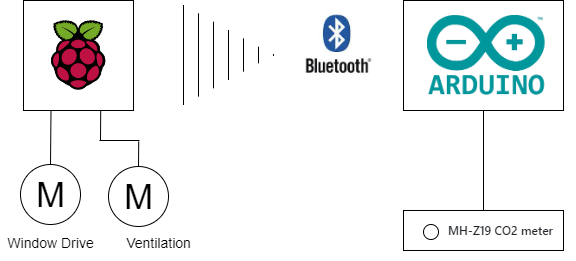
\includegraphics[height=50mm,left]{images/system}
	\centering
	\caption{system description}
	\label{fig:system}
\end{figure}






